\section{Verbesserungen} 
\label{Verbesserungen}

\paragraph{Temperatur}
Es wurde ein NTC mit 5\,\% bei 25\,°C Toleranz genommen, besser wäre 1\,\% gewesen, was nicht viel teurer wäre. Mit der gleichen Berechnung, jedoch mit einer anderen Toleranz, wie unter dem Kapitel \ref{Temperaturmessung}, wäre anstatt 19.3\,°C 20.0\,°C herausgekommen was eine Abweichung von 0.2\,°C bei Raumtemperatur ausmachen würde.

\paragraph{Genauigkeit}
Der ADC des ESP32 hat einige Tücken. So wurde zwar das Problem, dass Spannungen unter ca. 170\,mV nicht gemessen werden können mit einem Wiederstandnetzwerk gelöst. Aber es bleibt, das Problem, dass sich verschiedene ESP eine unterschiedliche Spannnungen unterschiedlich einlesen. Dies ist deswegen, weil die interne ADC-Referenzspannung des ESP32, zwar als 1100\,mV angegeben ist, in Wahrheit aber zwischen 1000\,mV und 1200\,V schwankt \cite{noauthor_analog_nodate}. Dies verdeutlicht die Abbildung \ref{pic: different_ADC}. Industriell lösen lässt sich dieses Problem, wenn man extra vorher kalibrierte ESPs kauft, bei welchen die Referenzspannung in das eFuse Vref gebrannt wurden. Dann kann über eine Funktion, die Referenzspannung ausgelesen werden. Besser wäre es 0\,dB Dämpfung für das einlesen einer Spannung zu benutzen, da diese auch wieder Toleranz behaftet ist. Diese interne Dämpfung macht nichts anderes als die angelegte  Spannung so stark zu Dämpfen, damit sie kleiner als die Referenzspannung ist. Aktuell ist der Standardwert von 11dB eingestellt. Ein weiteres Problem war, dass die Eingelesenen ADC-Werte sich unterscheiden, je nach dem wie belastet der ESP32 war. So wurde die Kurve \ref{pic: /ADC_Input_Kurve} mithilfe eines Testprogrammes aufgenommen, welches der ESP32 im Gegensatz zur richtigen Software nur gering belastet. Die Ausgabe per PWM, war ebenso Problematisch, denn die obere Amplitude war tiefer, wenn der ESP Belastet wurde, Ursache hierfür kann auch die Versorgungsspannung sein welche um 10m\,mV bei Belastung tiefer war.

\begin{figure}[h!]
	\centering
	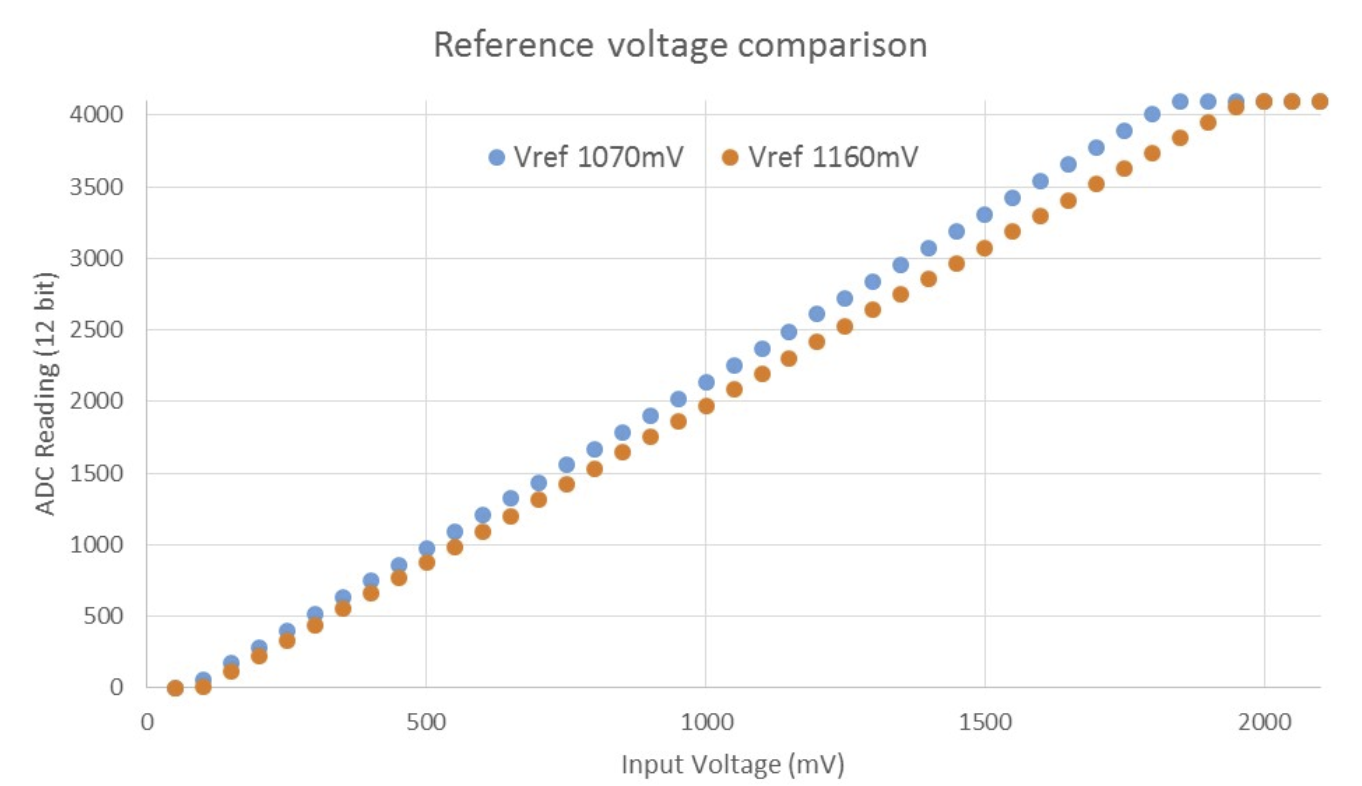
\includegraphics[width=\textwidth]{graphics/ADC_verschieden.png}
	\caption{ADC-Werte unterscheiden sich von ESP zu ESP unterscheiden \cite{noauthor_analog_nodate}}
	\label{pic: different_ADC}
\end{figure}
	
\paragraph{Zusammenstecken}
Man sollte darauf scheuen, dass die Frontplatte und der Hauptprint des Sensorbausteins richtig herum zusammengesteckt werden. Es hierzu zwar einen Markierungspunkt und Beschriftungen, die Eindeutig auf die Richtung hinweisen, besser wäre aber wenn es mechanisch nicht anders möglich wäre. Der Sensorbaustein wird durch ein falsches Zusammenstecken nicht beschädigt, nur die Funktion ist beeinträchtigt.
	
\paragraph{Beschriftung}
Beim Aktorbaustein ist die Beschriftung der Taster clear und mode vertauscht.

